\documentclass[12p,letterpaper]{article}
\usepackage[legalpaper,margin=1in]{geometry}
\usepackage{apacite}
\usepackage{varwidth}
\usepackage{graphicx}
%\usepackage{mathptmx} % Times New Roman Style
\usepackage{titlesec}
\usepackage{listings}
\usepackage{caption}
\usepackage{subcaption}
\usepackage{hyperref}
\providecommand\abstractname{Abstract}
\def\abstract{}
\def\endabstract{}
\renewenvironment{abstract}{%
  \centering\small
  \textbf\abstractname
  \list{}{\leftmargin2cm \rightmargin\leftmargin}
  \item\relax
}{%
  \endlist \par\bigskip
}

\makeatletter
\renewcommand\tableofcontents{%
  \null\hfill\textbf{\Large\contentsname}\hfill\null\par
  \@mkboth{\MakeUppercase\contentsname}{\MakeUppercase\contentsname}%
  \@starttoc{toc}%
}
\makeatother

\begin{document}
    
    \title{\vspace{-3.0cm}\Large{\textbf{Image Template Matching}}}
    \author{Gohur Ali \\ Computer Vision}
    \maketitle
    %\linespread{1.5}    
    \tableofcontents

	\pagebreak
    \section{Problem 1}
		
		\subsection{Algorithm}
			\begin{figure}[h]
				\centering
				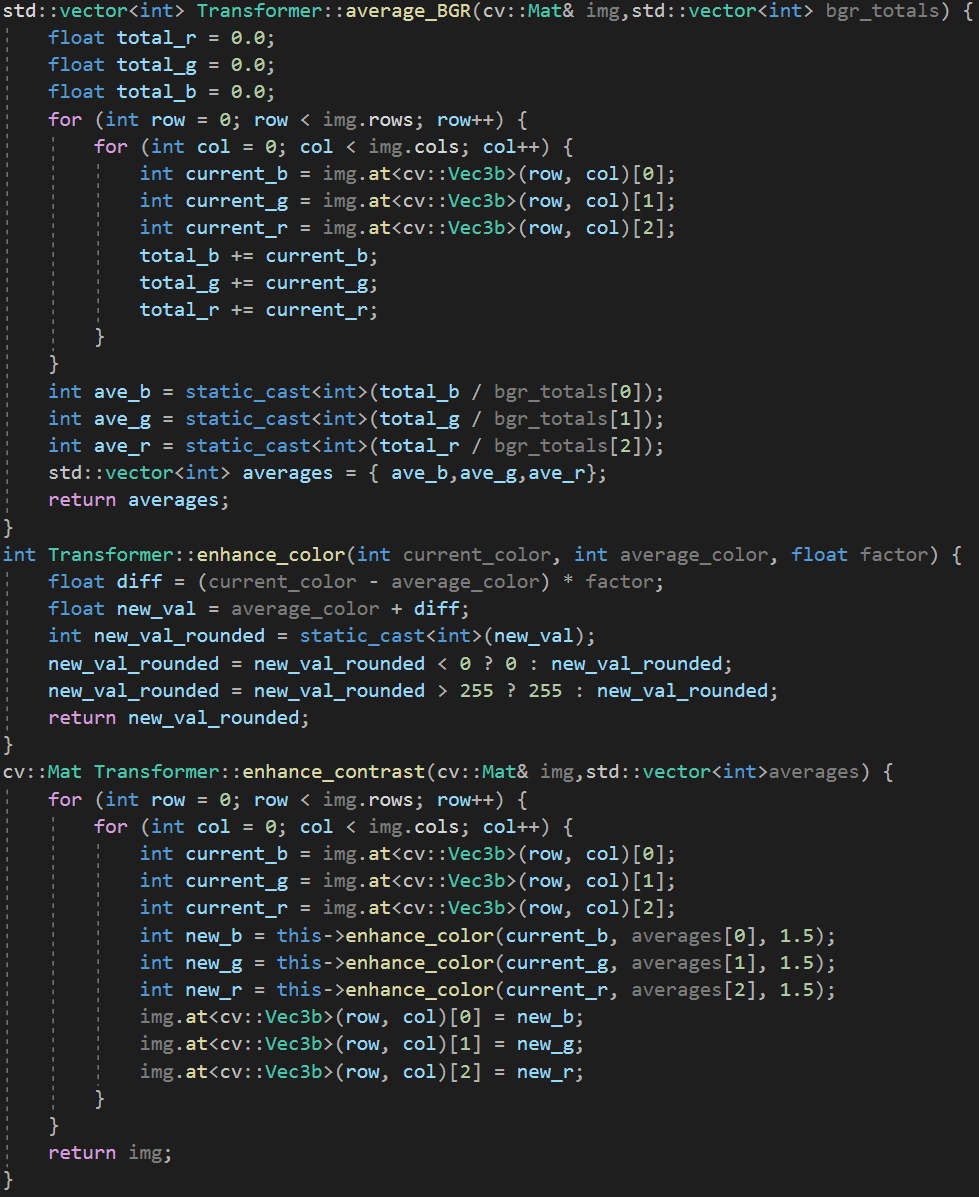
\includegraphics[width=10cm]{images/prob1_algo.PNG}
			\end{figure}
			
			\begin{figure}[h]
				\centering
				\begin{minipage}{.25\textwidth}
					\centering
					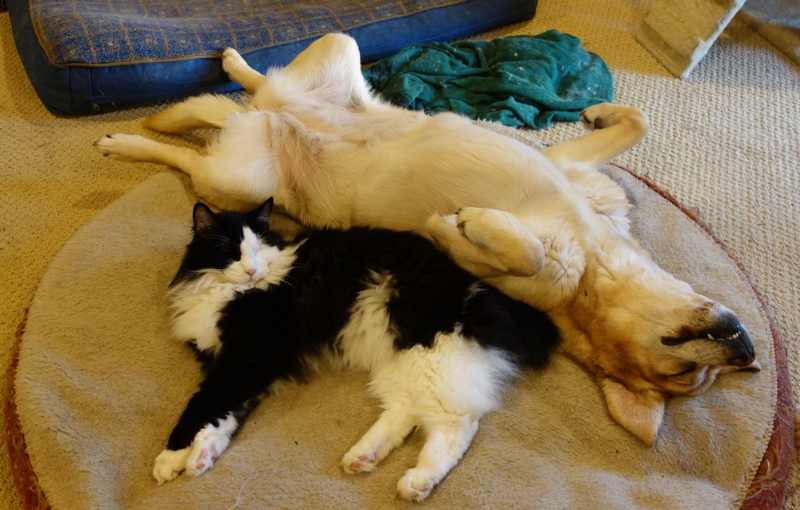
\includegraphics[width=5cm]{images/prob1_input.jpg}
					\caption{Input image}
				\end{minipage}
				\begin{minipage}{.5\textwidth}
					\centering
					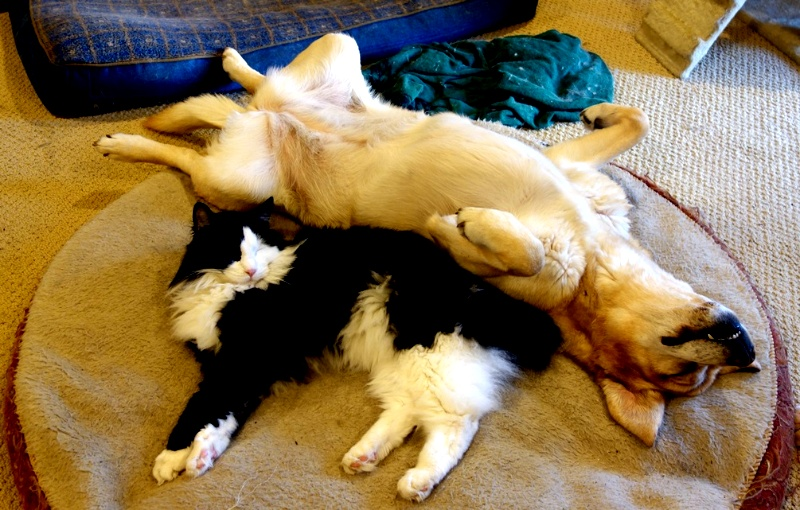
\includegraphics[width=5cm]{images/prob1_output.jpg}
					\caption{Output image}
				\end{minipage}
			\end{figure}

			\begin{figure}[h]
				\centering
				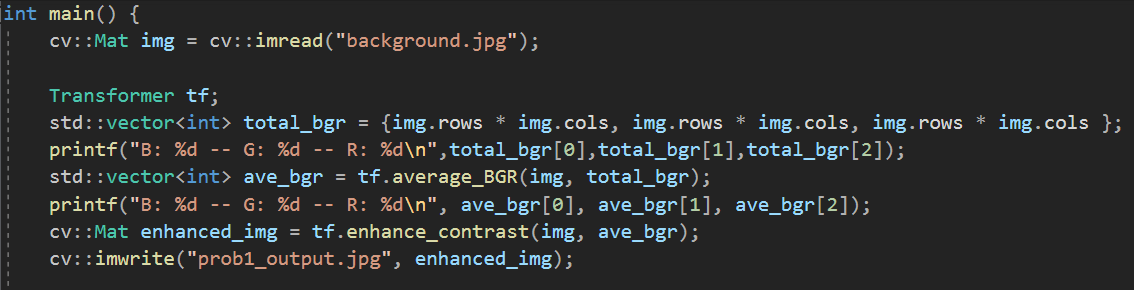
\includegraphics[width=10cm]{images/main1.PNG}
			\end{figure}
			
	\pagebreak
	\section{Problem 2}
		
		\subsection{Code}

			\begin{figure}[h]
				%\centering
				\hspace*{-0.8in}
				\begin{minipage}{0.63\textwidth}
					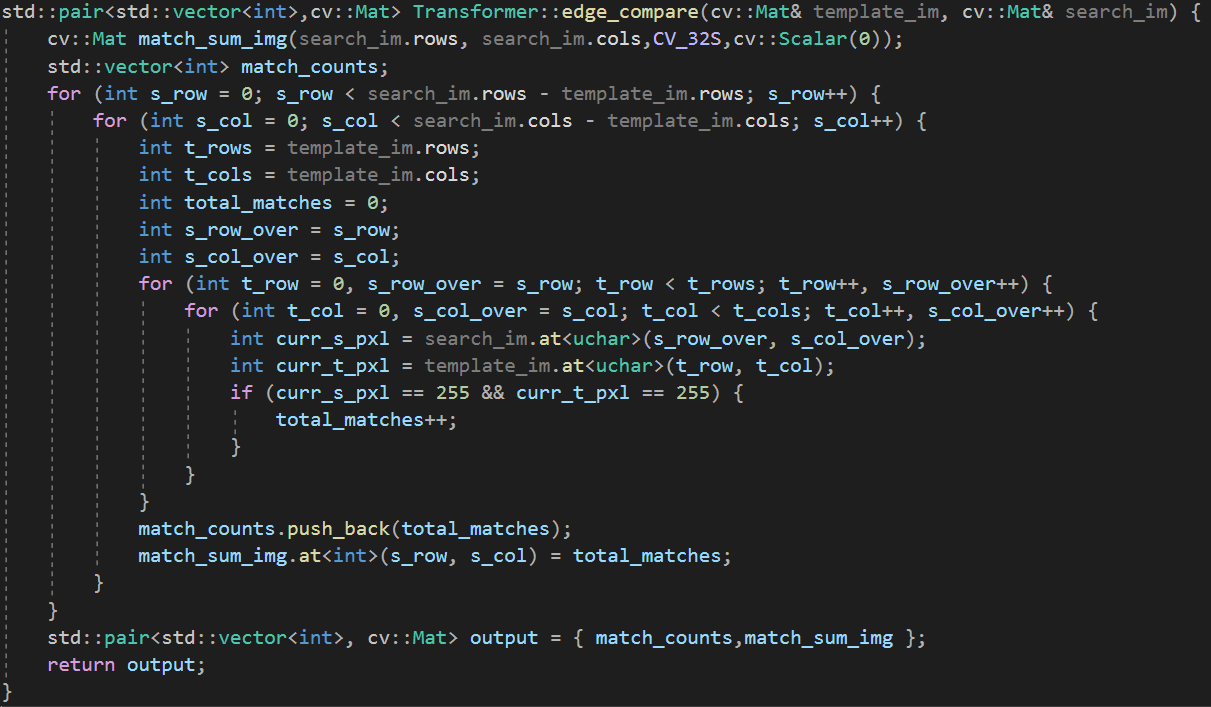
\includegraphics[width=10cm]{images/prob2_slidingwindow.PNG}
				\end{minipage}
				\begin{minipage}{0.63\textwidth}
					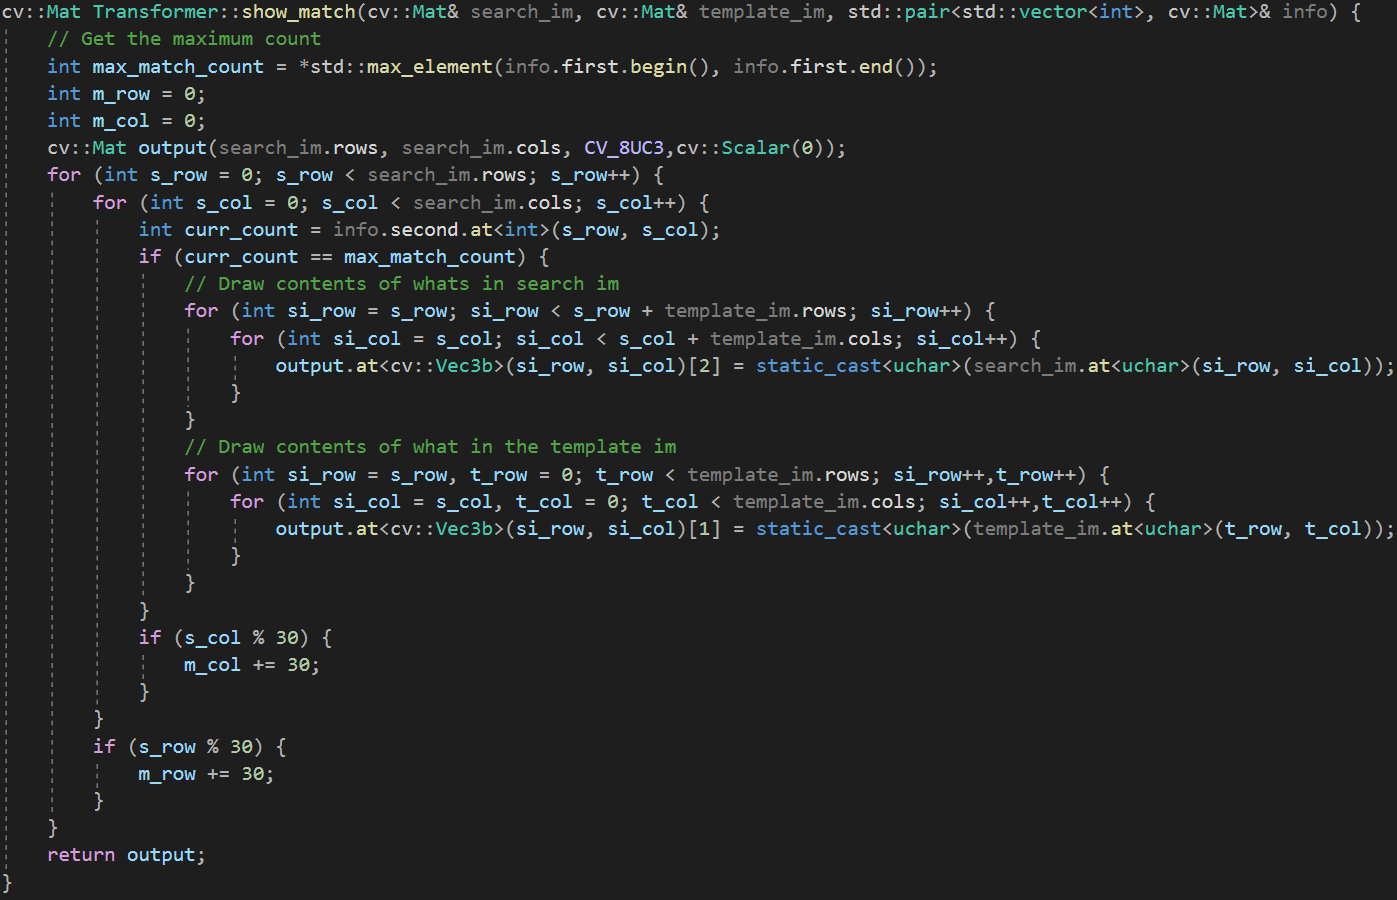
\includegraphics[width=10cm]{images/prob2_showimg.PNG}
				\end{minipage}
			\end{figure}
				
		\subsection{Results}
			\begin{figure}[h]
				\centering
				\begin{minipage}{0.35\textwidth}
					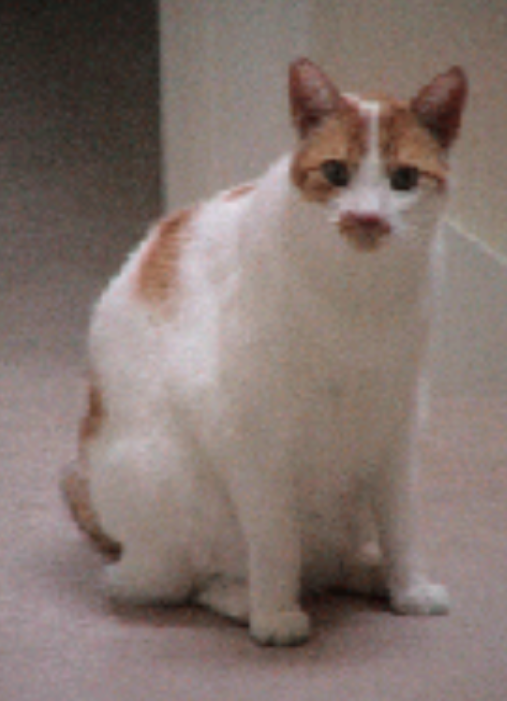
\includegraphics[width=4cm]{images/prob2_large.PNG}
				\end{minipage}
				\begin{minipage}{0.35\textwidth}
					
\includegraphics[width=4cm]{images/prob2_small.PNG}
				\end{minipage}
			\end{figure}

			\begin{figure}[h]
				\centering
				\begin{minipage}{0.25\textwidth}
					
\includegraphics[width=3cm]{images/search_im.PNG}
				\end{minipage}
				\begin{minipage}{0.25\textwidth}
					
\includegraphics[width=3cm]{images/template_im.PNG}
				\end{minipage}
				\begin{minipage}{0.25\textwidth}
					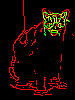
\includegraphics[width=3cm]{images/matches.PNG}
				\end{minipage}
				\caption{Resized and matched using sliding window approach}
			\end{figure}

			Using a sliding window method and calculating edge match
			counts, we can see that we find the location of the cat head in the
			search image. On the right most image, the red outline represents these
			search image, green being the template image, and yellow being direct
			matches.

		\subsection{Complexity}

			The complexity would be $O(n^{2} \cdot m^{2})$. This is because we first iterate
			through the search image which is and an $n \times n$ operation. Then within that, we
			iterate through the template image and calculate matching edges which is an $m \times m$
			operation.

		\subsection{Comparing to Convolution function}
			\quad The implementation shown above is similar to the convolution function. Rather 
			it is like a sliding window approach where the sliding window is the template image 
			over the search image. As the windows slides around the image, and any edges are
			overlapping are added to a match counter for each stride of the window. However,
			on the other hand, the convolution function performs a dot product with every stride.
			This would not perform the task needed where we need to determine how many edges 
			overlap with eachother. 

		\subsection{Greyscale Image Comparison}

			In order to compare greyscale images, one would need to compute pixel distances for position
			and intensity. In terms of this program, we would still utilize a sliding window approach, however,
			for each pixel in the window compute the distance for pixels with the same intesity and its position. 
			If they are within a certain threshold it will be matched. 

\end{document}